%!TEX root = ../Main.tex

\chapter{PolyMarker: A fast polyploid primer design pipeline.}
\chaptermark{PolyMarker}
\glsresetall
\label{cha:polymarker}
%\section{Introduction} 
%Explain how the SNP markers are designed without the tool and an overview. 
\section{Background.}


\gls{snp} are variations that occur in specific positions of the genome in at least 1\% of the population of certain species \citep{Jehan2006}. 
In modern breeding programs \gls{snp} markers are a prevalent technology to select individual plants or seeds containing a particular locus, which is linked to a trait (ie. a marker linked to a resistance gene, see Chapter \ref{yr15}). 
\glspl{snp} marker is a specific case of \gls{pcr} amplification where two competing sequences from different alleles are amplified. 
However, in polyploid species the variations between homoeologues are not considered \glspl{snp}.
Because of the similarity homoeologous regions can interfere in \gls{pcr} amplification it is preferable to design primers that will take in account the variations between the genomes and the target \gls{snp} simultaneously. 
This chapters describes PolyMarker, a bioinformatic tool to design genome-specific primers. 


\subsection{Primers and Polymerase Chain Reaction}
\label{sub:poly:pcr}
To generate new copies of DNA, biological systems require a DNA polymerase to copy DNA into DNA or a reverse transcriptase to translate RNA to DNA. During DNA replication, the DNA polymerase binds to the template strand and to a short strand of RNA that serves as a primer for DNA synthesis and replication, and then adds complementary nucleotides. Eventually, this results in two complementary DNA strands \citep{mullis1987process}.

This process can be used to generate multiple copies of a DNA sequence using the \gls{pcr}. 
PCR uses a heat-stable DNA polymerase to amplify the template sequence. 
The DNA polymerase requires a primer sequence that is complementary to the template strand to begin the reaction. Usually, chemically synthesised oligonucleotides of approximately 20 bases are added as primers (see Section \ref{sub:poly:primer3} for details on primer design). 
This primer sequence can be specific to the target region, or random if multiple regions are being duplicated. 
Once the DNA strand has been elongated, the temperature is elevated and then lowered to separate the DNA strands. 
The process is repeated multiple times to increase the number of DNA sequences exponentially \cite{alberts2014molecular}.

\Gls{pcr} amplification is a technique that can be used to copy a fragment of DNA several times. 
To start the amplification a pair of sequences (left and right primers) on each side of the target sequence is required. 
The sequence between primers is copied thanks to the DNA polymerase, an enzyme that moves along the DNA strand making a copy (product). 
The process starts with an increase in temperature in which the double stranded DNA when the DNA molecule is melted in individual strands. 
Then, the temperature is dropped so the primers anneal to the DNA strands. 
Depending on the reaction type the temperature is raised again to 72°C which is the temperature at which Taq polymerase extends. 
At this point, the polymerase starts extending the strand from the 3'-end of the primer. 
The temperature is raised again to separate the new strand from the original DNA and lowered again to get the right primer to anneal to the new product.
Then, in the extension step, the amplification occurs until the end of template sequence, were the 5'-end of the left primer was originally located. 
This process is repeated several times to increase the representation of the target DNA (Figure \ref{fig:poly:amplificationProduct}).  

\begin{figure}

\includegraphics[width=1\textwidth]{PolyMarker/Figures/intro/amplificationProduct.pdf}
\caption[PCR Diagram]{PCR Diagram. PCR is used to amplify a region of the DNA (green bar) target to amplify (product; red line) is found by a pair of primers (blue lines). The 3' and 5' represent the orientation of the primers.}
\label{fig:poly:amplificationProduct}
\end{figure}

\subsection{Primer design with Primer3}
\label{sub:poly:primer3}
To initialize de \gls{pcr} reaction (Section \ref{sub:poly:pcr})) it is crucial to design pairs of short DNA sequences, primers, that will start the amplification process. 
For a primer to be effective it has to be design under certain constrains. 
Primer3 \citep{Untergasser2012} is a bioinfrmatic tool to desig primers, considering the following critera:

\begin{description}
    \item[Oligonucleotide melting temperature]. It is the temperature at which the double stranded primer melts into single strands. If the melting temperature is too high, the primer will not bind to the target sequence \citep{Breslauer1986}.
    \item[Size.] The size of the primers needs to be balanced to be long enough to provide the desired specificity to the target seqnece, and short enough to to bind easily to the target sequence. A common range of sizes for priemrs is between 18-25bp. 
    \item[GC content.] Primers with a high GC content are more efficent, however they also tend to be less specific \citep{Rychlik1995}.
    \item[Avoid primer-dimers.] In a primer pair, if the corresponding 3' ends are similar the primer pairs may bind to each other. Hence, when selecting a primer pair, even if the individual primers are good candidates, the corresponding pair must be checked to avoid this issue. \citep{Chou1992}.
    \item[PCR product size.] It is the distance between the 5' end of both primers. The length of the product will determine how many cycles of extension are needed. For SNP markers, a short product size is prefered because the snp is already contained in the primer. 
    \item[Positional constrains in the template sequence.] It is possible to exclude or force the inclusion of certain regions in the primer design. In particular, this capability enables PolyMarker to select primers with the SNP in the 3' end of the first primer for KASP (see Section \ref{sub:poly:kasp}) and genome-specifc priemrs on the second primer (see Section \ref{sub:poly:genome-specific}). 
\end{description}
This list is of criteria considered by Primer3 is not comprehensive, but it includes the relevant options considered for primer design in PolyMarker. 

\subsection{KASP assays.}
\label{sub:poly:kasp}
A technology used for genotyping SNP markers is Kompetitive Allele Specific PCR (KASP) assay, the original target technology for PolyMarker.
The assay consists on triplets of primers, having a primer for each allele and a common primer that will amplify both alleles. 
The allelic primers have at the 5'-end a tail, HEX (5' GAAGGTCGGAGTCAACGGATT 3') or FAM (5' GAAGGTGACCAAGTTCATGCT 3'), which is used to distinguish between them (Figure \ref{fig:poly:kaspTriplet}). 
The KASP mix contains complementing oligos to the HEX and FAM tail, which contain a dye that is only visible when the corresponding allele has amplified. 
The intensity of each dye is used to measure relative amplification of each allele. 
In KASP assays, the distance between the left and right primers is kept as short as possible, to avoid having an extension step. 
As the primers are around 21-25bp, the minimum product size is between 42-50bp, with products rarely going over 75bp.  
Samples with the same genotype cluster: Samples on each axis correspond to homozygous individuals and samples clustered between the homozygous clusters are heterozygous (Figure \ref{fig:poly:kaspHet}). 
If the experiment fails, because poor amplification, that means that there are no distinguishable clusters amongst the samples (Figure \ref{fig:poly:kaspFail}; \citealt{LGC}).


\begin{figure}
\centering
    \begin{subfigure}{0.85\textwidth}
    \caption{}
    \label{fig:poly:kaspTriplet}
    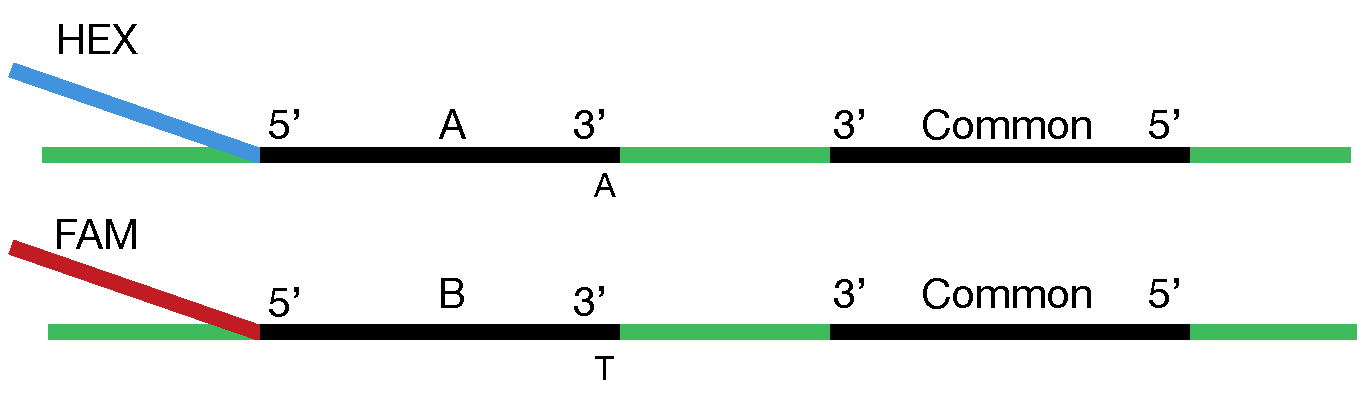
\includegraphics[width=1\textwidth]{PolyMarker/Figures/intro/kaspTriplet.pdf}
    \end{subfigure}

    \begin{subfigure}{0.45\textwidth}
    \caption{}
    \label{fig:poly:kaspHet}
    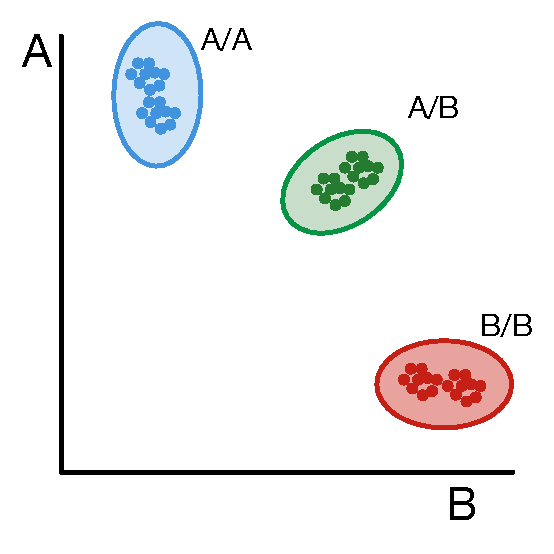
\includegraphics[width=1\textwidth]{PolyMarker/Figures/intro/kaspHet.pdf}
    \end{subfigure}
    ~
    \begin{subfigure}{0.45\textwidth}
    \caption{}
    \label{fig:poly:kaspFail}
    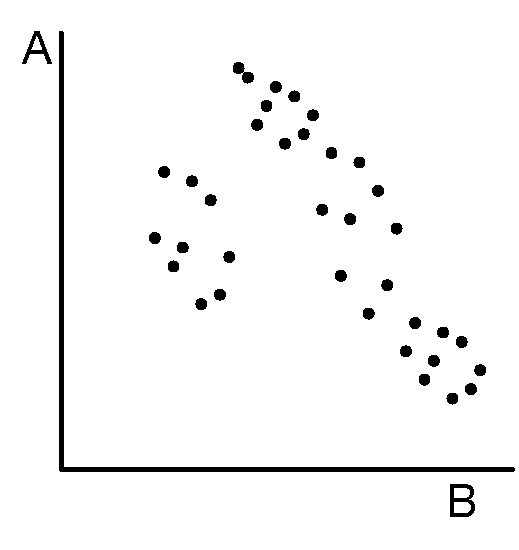
\includegraphics[width=1\textwidth]{PolyMarker/Figures/intro/kaspFail.pdf}
    \end{subfigure}

\caption[KASP Assays]{KASP Assays (\subref{fig:poly:kaspTriplet}) A KASP assay consists on three primers. Primers A and B are specific for certain allele and the HEX and FAM tails are added at the 5'-end on each primer. The common primer amplifies both possible products. The SNP is an A/T, the only difference between alleles. (\subref{fig:poly:kaspHet}) Ideal KASP results are obtained when tight and distinct clusters are obtained. The samples containing A allele clusters on the top-left (blue), the B allele cluster on the bottom-right (red) and the heterozygous cluster between the homozygous clusters (green). Each dot represent a sample and the axes are the relative intensity of amplification of each allele. (\subref{fig:poly:kaspFail}) KASP results in an experiment with inconsistent amplification between the two alleles, clear clusters between samples  are missing. }
\end{figure}


\subsection{Genome specific primers.}
\label{sub:poly:genome-specific}
One of the main challenges of working with polyploid species is the design of genome specific molecular markers. 
In hexaploid wheat, most of the genes have at three homoeologues copies, one for each genome (See section \ref{lit:polyploidy}). 
The similarity between homoeologues is around 98\% \citep{Krasileva2013}, which represent around 1 mismatch for every 50 bp. 
This means that a primer in a conserved region of 21 bases targets any of the homoeologues if it does not have variations on it.
In Figure \ref{fig:poly:pimerChrSpecificDiagram}, variations between genomes are represented with red lines, which are randomly distributed across homoeologues. 
The $\alpha$ is randomly generated using the sequence of chromosome 1D, however, because it doesn't have any variation specific to the D genome, products from it can amplify any of the genome. 
On the contrary, the $\beta$ starts with a base that is unique to the D genome, hence the product is genome specific. 

\begin{figure}
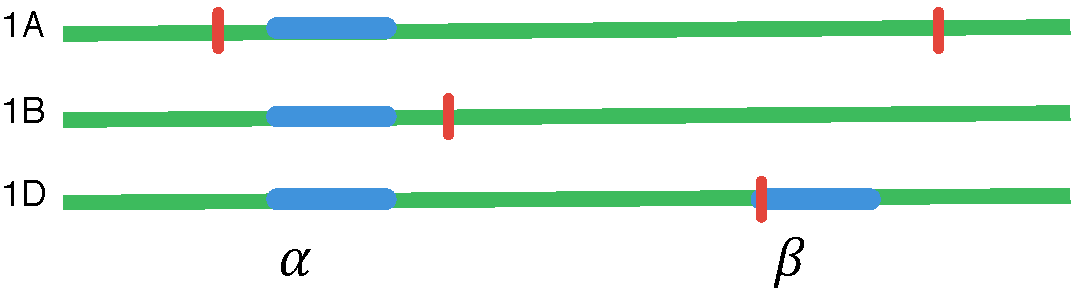
\includegraphics[width=1\textwidth]{PolyMarker/Figures/intro/primerChrSpecificDiagram.pdf}
\caption[Target of genome specific primer.]{Target of genome specific primer. Primers selected randomly (blue lines) can bind to any of the three homoeologous regions if they fall on regions without variations between them (red vertical lines). The $\alpha$ primer doesn't contain any variation between chromosomes, hence it will bind to the chromosomes 1A, 1B and 1D. The $\beta$ primer has a variation specific to the D genome, hence it will only amplify the 1D chromosome.}
\label{fig:poly:pimerChrSpecificDiagram}
\end{figure}

A variation between homoeologues in the primers is not enough to guarantee that the amplification is going to be genome specific. 
The polymerase is more specific to variations were the amplification starts, so variations in the 3'-end improve the specificity of primers \citep{Huang2010}. 
Hence, when designing genome-specific assays the specificity of the primers is scored according to the position of the variation as:  strong, when the variation is on the 3'-end; intermediate, when the variation is on the 2nd position; weak when the variation is on the 3rd position; and not specific when the variation occurs after the 3rd position (Figure \ref{fig:poly:3PrimeRules}).  

\begin{figure}
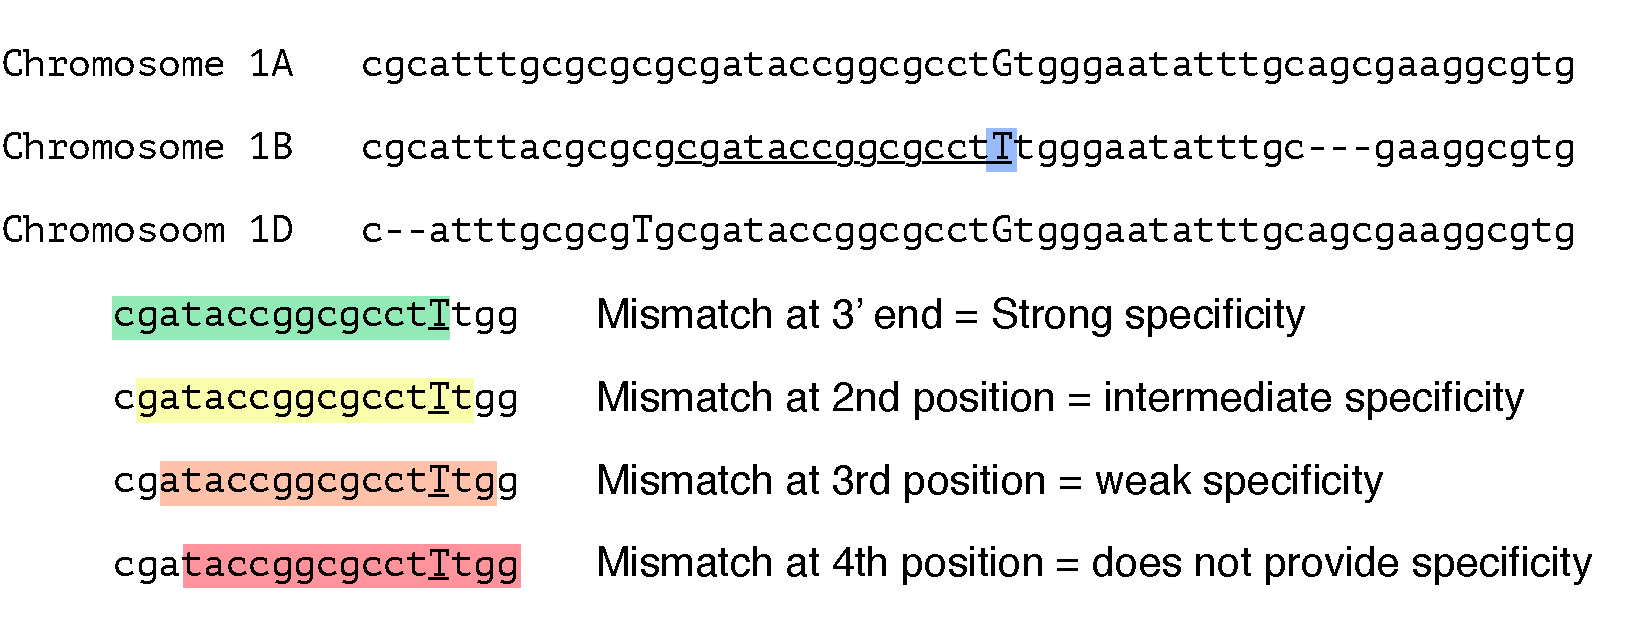
\includegraphics[width=1\textwidth]{PolyMarker/Figures/intro/specificPosition.pdf}
\caption[Effect of position of variation on primer specificity.]{Effect of position of variation on primer specificity. Several candidate primers to design a genome specific assay for chromosome 1B are shown. The T highlighted in blue is a variation unique to the target chromosome. The closer the T providing specificity is to the 3' of the primer, the more specific it is. }
\label{fig:poly:3PrimeRules}
\end{figure}


To ensure that all the constrains needed to produce genome-specific primer pairs, the following steps need to be done: 

\begin{enumerate}
\item First, a global alignment of the target sequence is used to find all the homoeologues and paralogues in the reference genome.
This is done with tools like \verb|blast| \citep{Altschul1990}, \verb|blat| \citep{Kent2002} or \verb|exonerate| \citep{Slater2005}.
All of these tools take a reference sequence and make an index of the database to speed up the search of the queried sequence  \ref{fig:poly:globalSearch}. 
Since some of the sources of SNPs come from transcriptome data and gene references, the original sequence may go over the intron-exon junction (see Section \ref{lit:rna-seq:lab}).  
The results are aligned to the target and may include sequences only from one exon, but not the adjacent intron, hence it is necessary to make a local alignment to ensure that corresponding bases are aligned correctly.

\begin{figure}
\centering
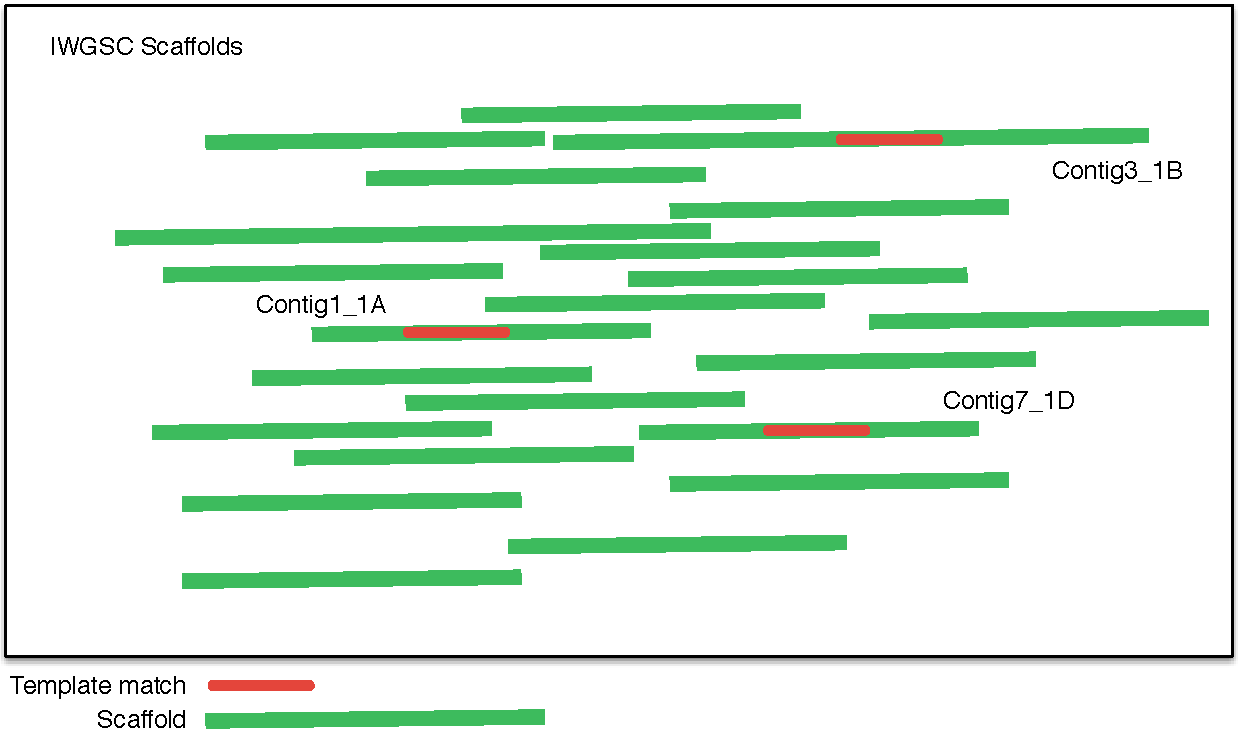
\includegraphics[width=1\textwidth]{PolyMarker/Figures/aln/scaffoldsSearch.pdf}
\caption{Global search of templates in the reference contigs.}
\label{fig:poly:globalSearch}
\end{figure}

\item To put all the sequences in the appropriate context, a local alignment is done (Figure \ref{fig:poly:globalAround}). 
This is done by extracting all the hits (matches) to the target reference and using a program like \verb|mafft| \citep{Katoh2013} or \verb|clustal| \citep{Higgins1988}. 
These tools are based on aligning all the possible sequences in pairwise combinations.
The distance between pairs is calculated to find which sequences are closer to each other, and then the process is repeated to refine the alignments until a consensus alignment is reached. 
This is useful on the context of genome-specific primer design because to correct the alignment on the presence of small \gls{indels}.  

\begin{figure}
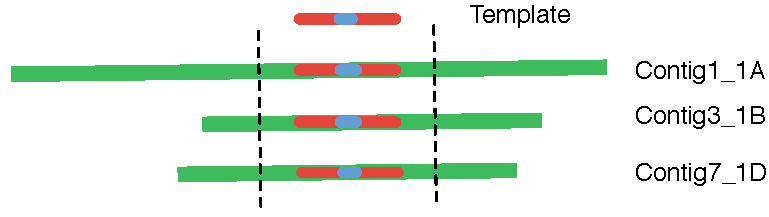
\includegraphics[width=1\textwidth]{PolyMarker/Figures/aln/scaffoldsFoundAround.pdf}
\caption[Selected regions around the SNP on every chromosome.]{Selected regions around the SNP on every chromosome. The blue line represents the position of the SNP.}
\label{fig:poly:globalAround} 
\end{figure}

\item Finally, the primers are validated to conform physicochemical properties that ensure the amplification. 
The melting temperature needs to be in the range were the DNA will separate, but not too high that the temperature will damage other elements in the reaction, such as the polymerase. 
Also, the primers must avoid sequences that self-bind, hairpins, or binding to the complementary primer. 
The validation primers based on their intrinsic properties can be done with tools like \verb|Primer3| \citep{Rozen}. 
%\unsure{If possible, expand and add diagram}
\end{enumerate}

\subsection{Objective.}

Most of the steps required to design genome-specific primers require different bioinformatic tools and the rules to improve the efficiency of the primers are established.
The objective of PolyMarker is to automate the primer design process, from a reference genome and a list of \glspl{snp} and produces genome-specific primers.
The pipeline has been published in \citet{Ramirez-Gonzalez2015a}.

\section{Pipeline. }
PolyMarker is an automated pipeline that takes as input a list of SNPs and a reference file and produces a list of primer triplets for SNP genotyping. 
The list of SNPs is first converted to a \verb|FASTA| file with ambiguity codes \citep{Cornish-Bowden1985} 
The template sequences are aligned with \verb|exonerate| \citep{Slater2005}  to find the homoeologous and paralogue regions to the target sequence.
For my thesis, I implemented this using the IWGSC reference sequence (described in Chapter \ref{lit:wheatResourcers}).  
Then, the alignment between homoeologues is refined using \verb|MAFFT| \citep{Katoh2013}. 
A list of candidate variations is produced and used as input for \verb|Primer3| \citep{Rozen}. 
Finally, the output of \verb|Primer3| is parsed to select the shortest primer pair containing the targeted SNP and a base that is specific to the target genome (Figure \ref{fig:poly:pipeline}).  
The pipeline is written as a Ruby script, using parsers and wrappers from BioRuby \citep{Goto2010} and bio-samtools \citep{Etherington2015,Ramirez-Gonzalez2012}. 
The software is open source and released as a biogem \citep{Bonnal2012}, \verb|bio-polyploid-tools|, the source code is available in: \url{https://github.com/TGAC/bioruby-polyploid-tools}.

\begin{figure}
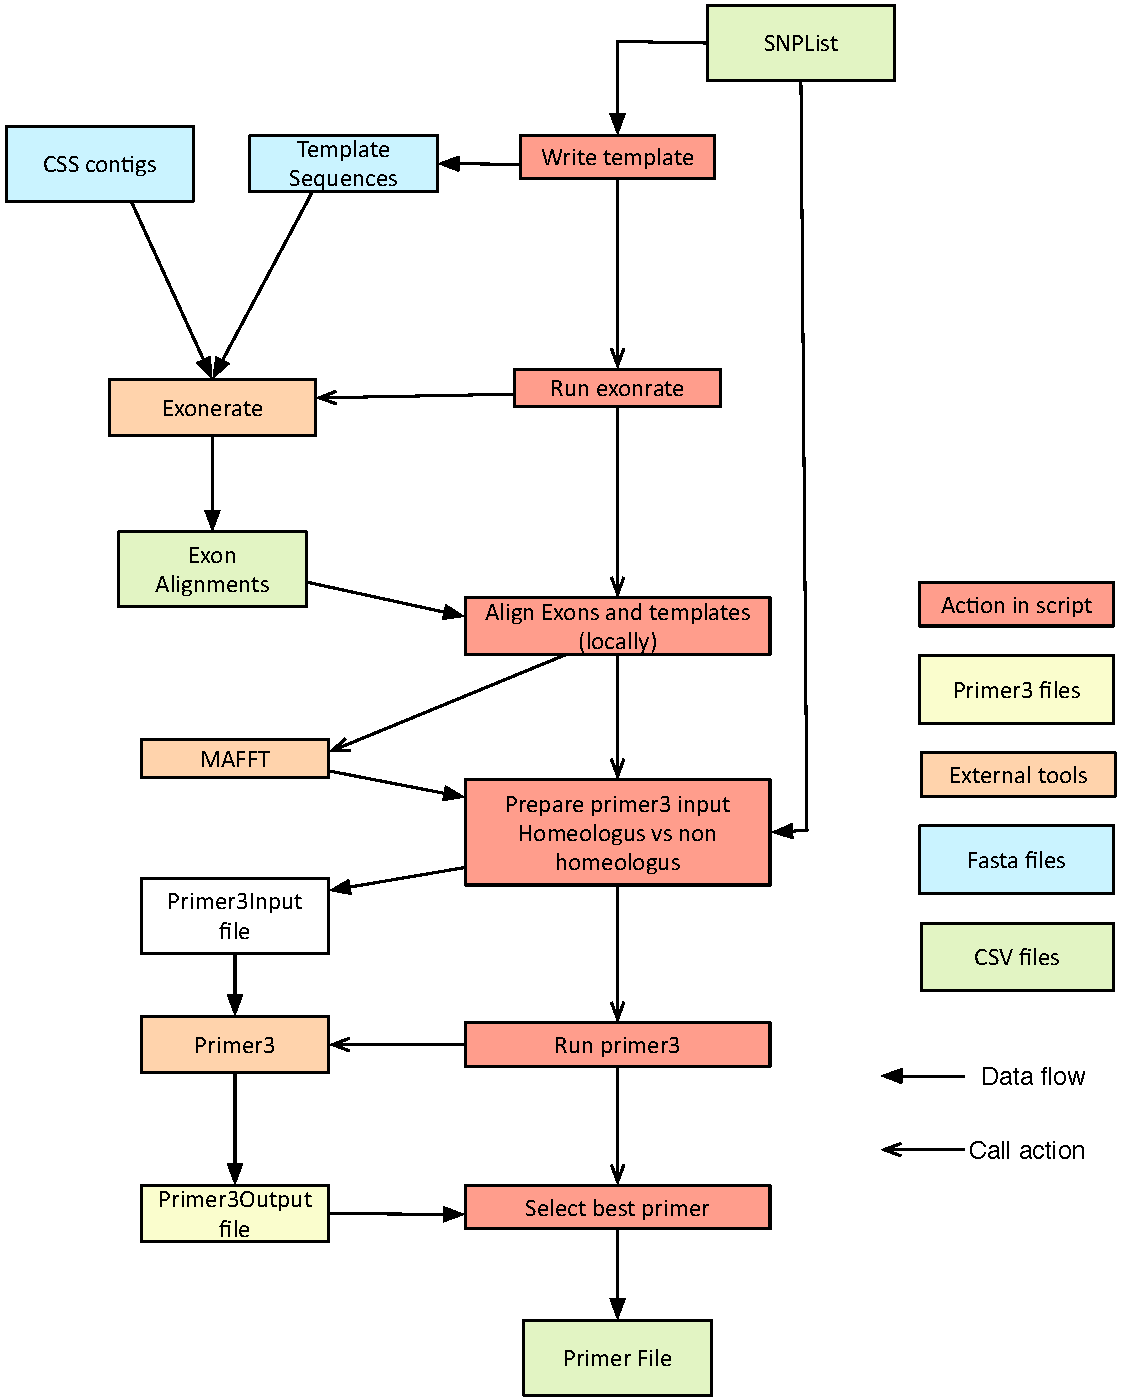
\includegraphics[width=1\textwidth]{PolyMarker/Figures/pipeline.pdf}
\caption[Steps and tools called by PolyMarker]{Steps and tools called by PolyMarker. The colours of the boxes represent: the step is an action inside the script(red); actions of the script(light red); temporary files(yellow); inputs(blue) and; outputs(green)}
\label{fig:poly:pipeline}
\end{figure}

The PolyMarker input consists on SNP list with: unique name for the marker, the target chromosome and the sequence for the marker. 
The alternative alleles are flanked by square brackets within the sequence. PolyMarker can take a list of several markers and design them in batch (Figure \ref{fig:poly:input}). 
A \verb|FASTA| file is produced with all the template sequences, with the alternative alleles substituted by the IUAPC ambiguity codes \citep{Cornish-Bowden1985}. 
The flanking sequence surrounding the SNP is limited by default to 100bp to reduce the search time and avoid missing regions that diverge near the SNP, as when the variation is near an intron-exon junction. 
The limitation of the flanking sequence to +/- 100 is consistent with the marker assay which is restricted to amplicons of 100-120 bp. 

%%TODO: Should we elaborate more here? 
\begin{figure}
    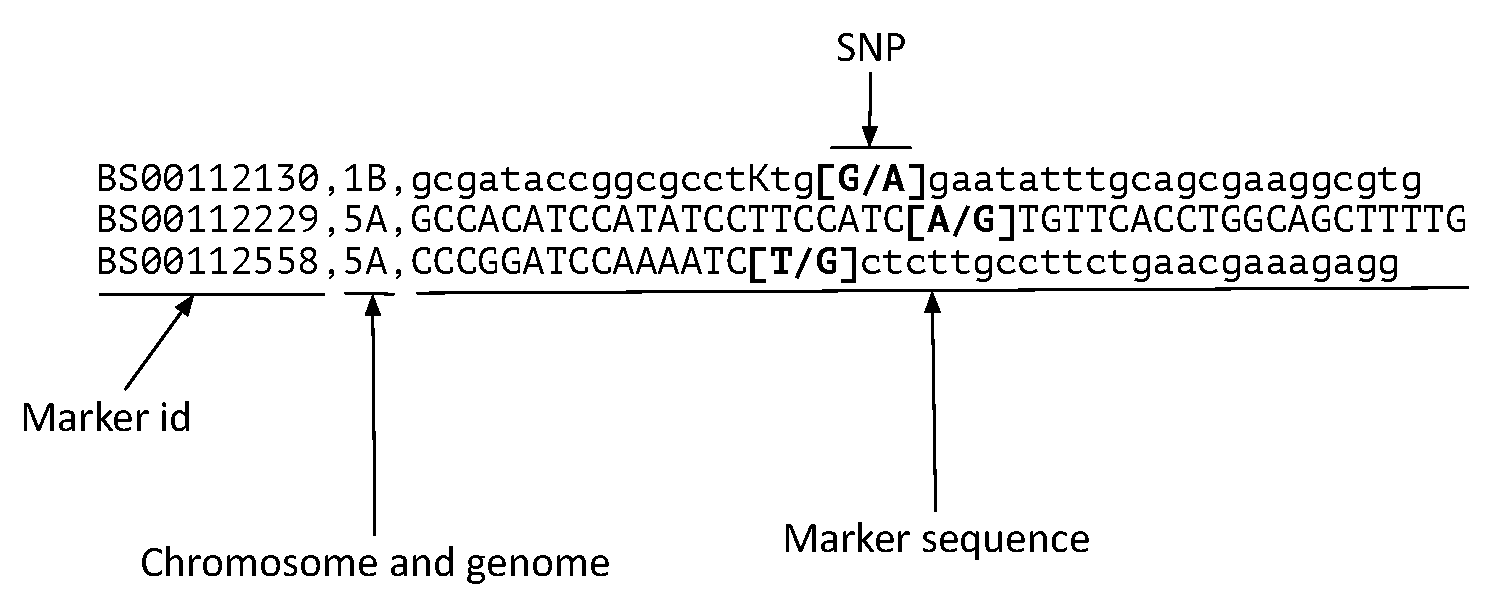
\includegraphics[width=1\textwidth]{PolyMarker/Figures/aln/input.pdf} 
      \caption[PolyMarker input]{PolyMarker input. The alternative alleles are surrounded by brackets. The rest of the figures are based on BS00112130, renamed as SNP-1.}
    \label{fig:poly:input}
\end{figure}

The template sequences are aligned to the reference using \verb|exonerate| (\citealt{Slater2005}; Figure \ref{fig:poly:globalSearch}). 
The following parameters are used to optimise the output:

\begin{description}

\item[\texttt{--verbose 0 --show --alignment no --show vulgar no}.] To override the default output. 
\item[\texttt{--bestn 20}.] By default, it increases the number of best hits to 20. Intuitively, it would be expected to have 3 copies, on for each homoeologue. However, the \acrshort{css} assembly has some duplication in the scaffolds and it is possible to find paralogues elsewhere in the genome. 
\item[\texttt{--model est2genome}.] To allow the search of sequences coming from transcripts, such as the SNPs described in Chapter \ref{yr15}  and in the SNP chip described by \citep{Allen2011}
\item[\texttt{--ryo 'RESULT:\char`\\t\%S\char`\\t\%pi\char`\\t\%ql\char`\\t\%tl\char`\\t\%g\char`\\t\%\char`\\n'}.]To set the output in a tabular format that is easy to parse as follow: \verb|\%S| the minimum information of the alignment, \verb|\%pi| percentage of identity, \verb|\%ql| query length, \verb|\%tl| target length and, \verb|\%g| orientation. 
\end{description}


All the hits that contain the SNP and have a percentage of identity over 90\% are extracted, this threshold allows to match homoeologs and paralogs. 
The coordinate of the SNP is calculated and 100bp on each flank are extracted by default, a reasonable product size for KASP assays. 
The flanking sequence may contain \acrshort{indels} and the sequences do not align naturally (Figure \ref{fig:poly:globalSequence}).
The following parameters can be adjusted to extend the functionality of PolyMarker: Minimum Identity to designs for organisms with homoeologous regions that are more divergent; flanking sequence for different types of primers (ie. for Sanger sequencing) and;  \verb|model| to adjust the search according to the source of the SNP (ie. if it is known that the SNP comes from DNA, \verb|affine:local| would be a better option as \verb|exonerate| will not pay attention to the intron-exon junctions).

\begin{figure}
\centering
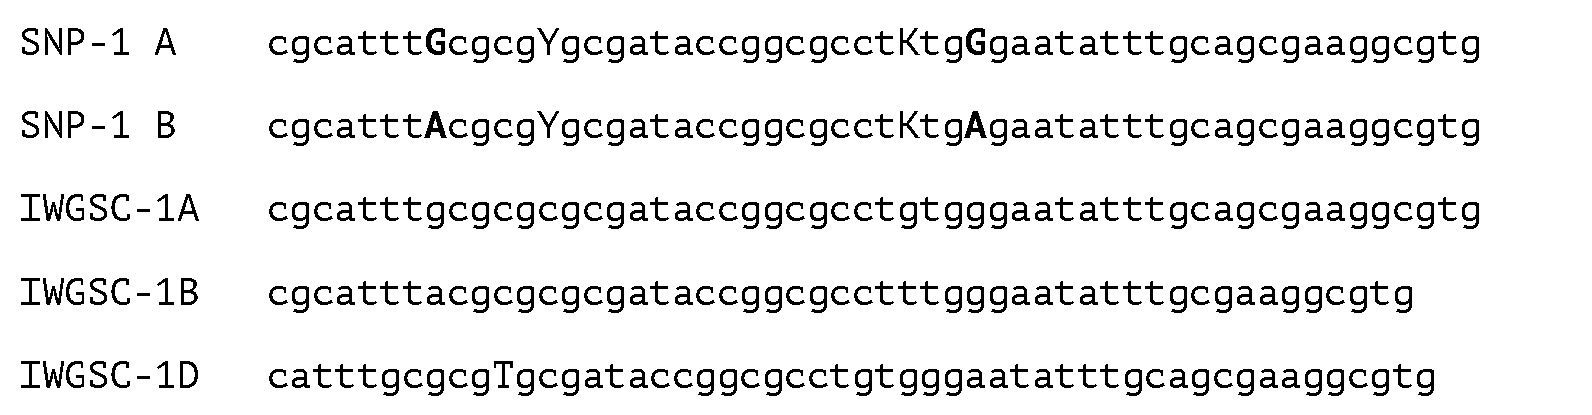
\includegraphics[width=1\textwidth]{PolyMarker/Figures/aln/scaffoldsFound.pdf}
\caption[Sequence of flanking regions around the SNP.]{Sequence of flanking regions around the SNP. The \acrshort{indels} produce a slight shift on the sequence.}
\label{fig:poly:globalSequence}
\end{figure}


%\unsure{Maybe explain the architecture before getting to the pipeline, or after}
Each SNP marker is represented on the \verb|Bio::PolyploidTools::SNP| class, containing the flanking sequence, the position of the SNP, multiple alignments and primers. 
For each step step there is a container that holds the SNP set and parses each output for all the called programs. 
The container for exonerate is \verb|BIO:PolyploidTools::ExonContainer|. 
The hits with the SNP are called exon henceforth, as the original design was for SNPs in gene models which may contain intron-exon junctions. 
The main job of the \verb|ExonContainer| is to parse the \verb|exonerate| output and add it to the corresponding SNP (Listing \ref{lst:poly:exonerateParsing}). 

\begin{code}[language=Ruby,caption={[\texttt{Bio::PolyploidTools::ExonContainer.add\_alignments}]Method in \texttt{Bio::PolyploidTools::ExonContainer} that adds to each SNP object the alignments}, label=lst:poly:exonerateParsing]
def add_alignments(opts=Hash.new) 
  opts = {:min_identity=>90 }.merge!(opts)
  exonerate_filename = opts[:exonerate_file]
  File.open(exonerate_filename) do |f|
    f.each_line do | line |
      record=Bio::DB::Exonerate::Alignment.parse_custom(line)
      if record and record.identity>=opts[:min_identity]
        snp_array = @snp_map[record.query_id]
        snp_array.each do |snp|                            
        if snp.position.between?( (record.query_start + 1) , record.query_end)
          exon=record.exon_on_gene_position(snp.position)
          snp.add_exon(exon, arm_selection.call(record.target_id))
        end
      end
    end
  end
end
\end{code}

Each \verb|SNP| contains a Hash to the best alignment to each chromosome, based on identity. 
When the \verb|ExonContainer| adds an alignment, the \verb|SNP| verifies that is the best hit for a given chromosome, to avoid scaffolds with duplicated sequences (Listing \ref{lst:poly:bestScaffold}).

\begin{code}[language=Ruby,caption={[Bio::PolyploidTools::SNP.add\_exon]Method in \texttt{Bio::PolyploidTools::SNP} that adds an alignment }, label=lst:poly:bestScaffold]
def add_exon(exon, arm)
  @exon_list[arm] = exon unless @exon_list[arm]
 @exon_list[arm] = exon if exon.record.score > @exon_list[arm].record.score
end
\end{code}

As it is common to have different conventions over different references on how the chromosomes are named, PolyMarker can be easily extended to parse different naming conventions. 
To achieve this, when the \verb|ExonContainer| is initialised a parsing function is set up. 
Then, when each alignment is added, the ID of the target sequence is parsed using the custom function (Listing \ref{lst:poly:exonerateParsing}, line 12).
An example of parsing functions for a chromosome are in Listing \ref{lst:poly:chromsomeParsing}.


\begin{code}[language=Ruby,caption={[Function that assigns a chromosome] Example function that assigns a chromosome from the two first letters of the scaffold}, label=lst:poly:chromsomeParsing]
arm_selection_functions[:arm_selection_first_two] = lambda do | contig_name |
  ret = contig_name[0,2]       
  return ret
end
\end{code}

%\pagebreak 
To ensure that the \acrshort{indels} between homoeologues do not produce spurious mismatches a local alignment is produced with \verb|MAFFT| (Figure \ref{fig:poly:localSequence}). 
The arguments used are the recommended ones in the manual for small number of sequences:

\begin{figure}
\centering
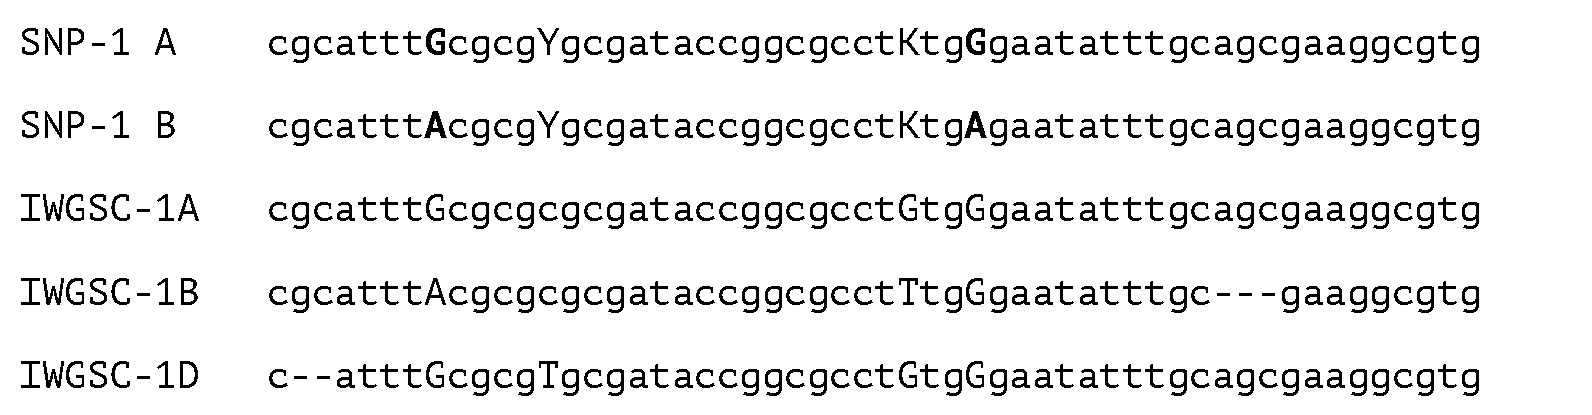
\includegraphics[width=1\textwidth]{PolyMarker/Figures/aln/localAlignment.pdf}
\caption{Local alignment on regions around the SNP detects \acrshort{indels}.}
\label{fig:poly:localSequence}
\end{figure}

\begin{description}
\item[\texttt{--maxiterate 1000}.] The local alignment is defined up to 1000 times.
\item[\texttt{--localpair}.] Compares all the possible pairs of alignment to each other
\item[\texttt{--quiet}.] To reduce the size of the logs.  
\end{description}

The class \verb|Bio::PolyploidTools::SNP| has the method \verb|aligned_sequences| which executes \verb|MAFFT| for the best hit on each chromosome to the marker. 
The first time it is invoked it stores the result as an attribute (Listing \ref{lst:poly:mafft}).
This approach hides the execution of the local alignment as an attribute and it avoids executing it several times when calculating the variations between homoeologues. 

\begin{code}[language=Ruby,caption={[\texttt{Bio::PolyploidTools::SNP.aligned\_sequences}]Method in \texttt{Bio::PolyploidTools::SNP} that calculates the local alignment}, label=lst:poly:mafft]
def aligned_sequences
  return @aligned_sequences if @aligned_sequences
  options = ['--maxiterate', '1000', '--localpair', '--quiet']
  mafft = Bio::MAFFT.new( 'mafft' , options)
  report = mafft.query_align(sequences_to_align)
  @aligned_sequences = report.alignment
  @aligned_sequences
end
\end{code}


PolyMarker searches across each base in the local alignment to identify the variations across homoeologues and the target marker.
A mask is produced to highlight the bases with a variations, Figure \ref{fig:poly:mask}, on the following categories:
\begin{labeling}{Non-homoeologous}
%\begin{description}[align=right,labelwidth=4cm]
\item [Specific] Homoeologous polymorphism which is only present in the target genome (upper case).
\item [Semi-specific] Homoeologous polymorphism is found in 2 of the 3 genomes, hence it discriminates against one of the off-target genomes or when not all the homoeologous sequences were found (lower case).
\item [Non-specific] No variation is found across homoeologues (\texttt{-}).
\item [Homoeologous] The target SNP is present across different chromosomes, so candidate SNP markers on this category are not expected to be reliably identifying the allele as these are not necessarily varietal polymorphisms (\texttt{:}).
\item [Non-homoeologous] The target SNP is not present across chromosomes, so it is most likely a varietal polymorphism which can be used to identify alternative alleles in the position (\texttt{\&}).
%\end{description} 
\end{labeling} 


\begin{figure}
\centering
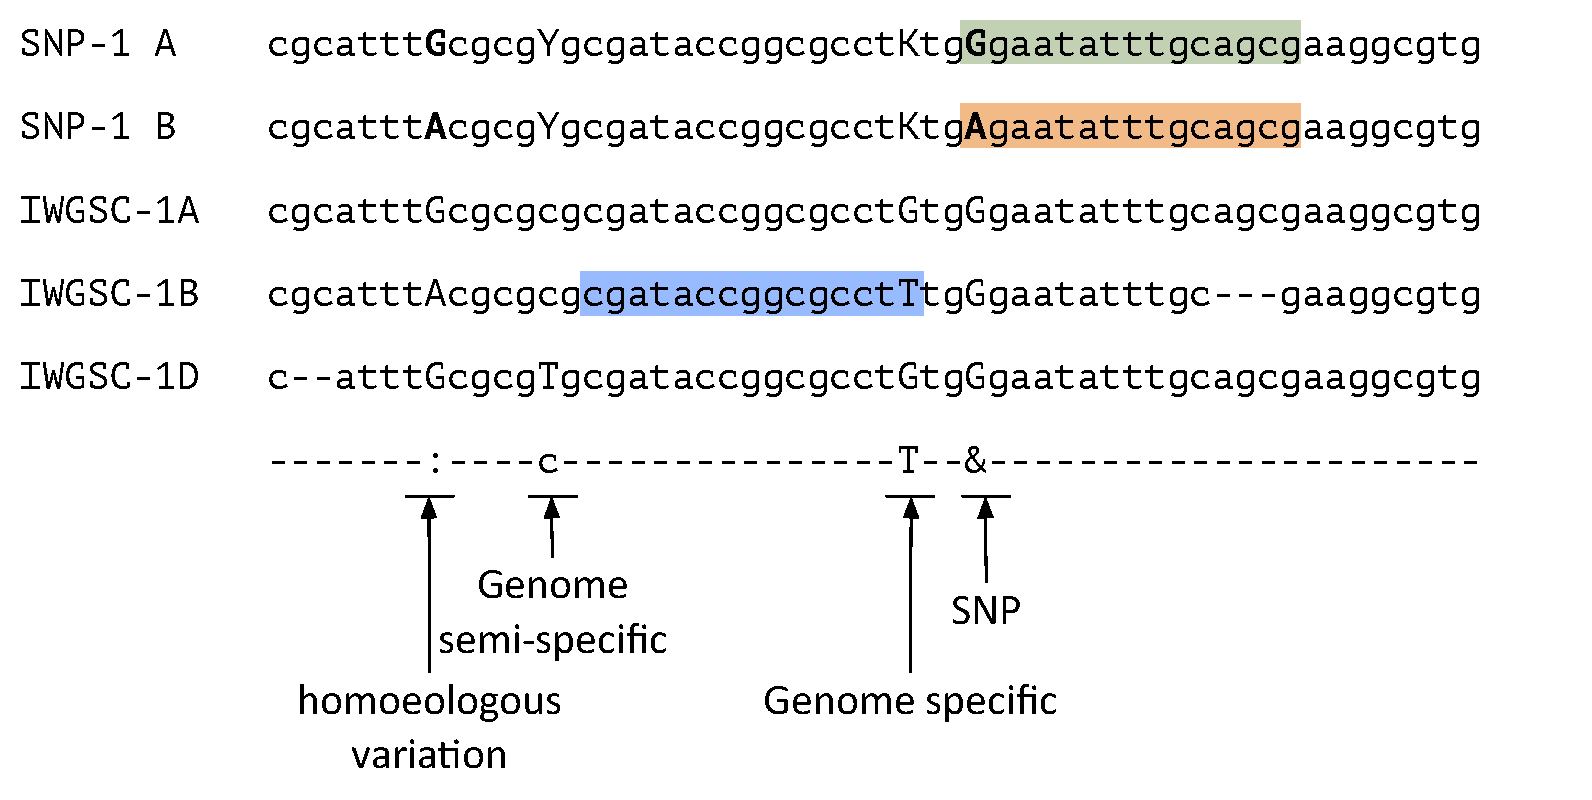
\includegraphics[width=1\textwidth]{PolyMarker/Figures/aln/mask.pdf}
\caption[Alignment with mask and primer candidates.]{Alignment with mask and primer candidates. The green and light red boxes highlight the allele specific primers. The blue box highlights a genome specific primer. }
\label{fig:poly:mask}
\end{figure}

To generate the mask the following logic is followed:
\begin{enumerate}
\item The aligned sequence of the target chromosome is set up as the default mask (Listing \ref{fig:poly:mask}, line 5).
\item Then each position in the mask is iterated base per base (Listing \ref{fig:poly:mask}, line 7).
\item A count of how many bases are the same across the chromosome and how many from the same chromosome group (defined by the first letter in the parsed chromosome) and how many chromosomes have local alignment (excluding \acrshort{indels}; lines 9-18).
\item  A position is labelled as uninformative (\verb|-|) when the position does not have any different bases, the sequence is only available from the target chromosome or there are unknown bases on that particular position (any chromosome has an \verb|N| on the given position; line 19).
\item When no alignment is present at all, the mask is filled with \verb|*| (line 20). This allows to identify the cases where only the initial marker sequence is available.
\item If the target chromosome has an unique variation, the base is converted to upper case (line 22). This implicitly leaves as a lower case the semi-specific variations. The \verb|genomes_count| is a variable set at initialisation time and keeps track of the number of expected alignments from the target group. This allows to use the same code for any level of polyploidy.  
\item At the position of the SNP, the special symbols are setup (lines 23-30)
\begin{enumerate}
\item By default, the SNP position is labelled as \verb|&| (line24).
\item All the observed bases, except the one in the target chromosome, are collected and converted to an IAUP ambiguity code \citep{Cornish-Bowden1985} (lines 26-28). If the bases in the SNP are contained in the ambiguity code the SNP is marked as homoeologous (\verb|:|; line 29)
\end{enumerate}
\end{enumerate}

When designing SNP markers the aim is to have the amplification as specific as possible. 
To improve the specificity of the assays, PolyMarker categorises all the possible primers as Specific; Semi-specific or; Non-specific. 
The candidate primer pairs are then evaluated with \texttt{Primer3} \citep{Rozen}. 
\texttt{Primer3} receives a file with the preferences to design the markers, for PolyMarker the following preferences are set up: 

\begin{description}
\item[\texttt{PRIMER\_PRODUCT\_SIZE\_RANGE=50-150}.] A reasonable size for KASP markers, as the technology does not have an extension step. 
\item[\texttt{PRIMER\_MAX\_SIZE=25}.] KASP primers are usually between 21 and 25 bases.
\item[\texttt{PRIMER\_LIB\_AMBIGUITY\_CODES\_CONSENSUS=1}.] To ensure that bases with ambiguity code are matched between primer pairs. 
\item[\texttt{PRIMER\_LIBERAL\_BASE=1}.] To allow the use of ambiguity codes in the sequence
\item[\texttt{PRIMER\_NUM\_RETURN=5}.] The maximum number of primer candidates. 
\end{description}
To design a different kind of primers it is possible to have a different set of preferences by feeding a standard \texttt{Primer3} preferences file with the option \verb|--primer_3_preferences FILE|. 

The input file for \verb|primer3| also include the template sequences with an ID. 
To keep track of what kind of marker each position will produce the ID field has the name of the primer and the specificity of the starting position of the common primer. 
The starting position of the primers is forced with the options \verb|SEQUENCE_FORCE_LEFT_END| and \verb|SEQUENCE_FORCE_RIGHT_END| on the specific and semi-specific positions. 
For the non specific positions only the \verb|SEQUENCE_FORCE_LEFT_END| is given to make a full search of candidates. 

\begin{code}[language=Ruby,caption={[\texttt{Bio::PolyploidTools::SNP.}\texttt{mask\_aligned\_chromosomal\_snp}] Method in \texttt{Bio::PolyploidTools::SNP} that calculates the mask of the alignment}, label=lst:poly:mask]
def mask_aligned_chromosomal_snp(chromosome)
  names = exon_sequences.keys
  parentals =  parental_sequences.keys
  local_pos_in_gene = aligned_snp_position
  masked_snps = aligned_sequences[chromosome].downcase
  i = 0
  while i < masked_snps.size
    different = cov = from_group = Count = 0
    names.each do | chr |
      if aligned_sequences[chr] and aligned_sequences[chr][i]  != '-'
        cov += 1 
        nCount += 1 if aligned_sequences[chr][i] == 'N' or  aligned_sequences[chr][i] == 'n' 
        from_group += 1 if chr[0] == chromosome_group
        if chr != chromosome 
          different += 1  if masked_snps[i].upcase != aligned_sequences[chr][i].upcase 
        end
      end
    end
    masked_snps[i] = '-' if different == 0 or if cov == 1 or nCount > 0
    masked_snps[i] = '*' if cov == 0
    expected_snps = names.size - 1 
    masked_snps[i] = masked_snps[i].upcase if different == expected_snps and from_group == genomes_count
    if i == local_pos_in_gene
      masked_snps[i] = '&'
      bases = ''
      names.each do | chr | { bases << aligned_sequences[chr][i]  if aligned_sequences[chr] and aligned_sequences[chr][i]  != '-' }
      code_reference = 'n'
      code_reference = Bio::NucleicAcid.to_IUAPC(bases) unless bases == ''
      masked_snps[i] = ':' if Bio::NucleicAcid.is_valid(code_reference,   original) and Bio::NucleicAcid.is_valid(code_reference,   snp)
    end
  i += 1
  end
  masked_snps
end
\end{code}

The class \texttt{Bio::DB::Primer3::Primer3Record} is used to keep the details of all the primers generated by \verb|primer3| for each template. 
In order to prioritise which primer is selected as the best primer on for each SNP, each \verb|Primer3Record| is scored according to their type and the product length (Listing \ref{lst:poly:score}).
By default, more priority is given to the specific, semi-specific and non-specific primers, in that order. 
In case of having more than one primer pair with the same specificity, the one with the shortest product length is chosen (Listing \ref{lst:poly:defScore}).  


\begin{code}[language=Ruby,caption={[\texttt{Bio::DB::Primer3::Primer3Record.score}]Method that calculates the score of a primer \texttt{Bio::DB::Primer3::Primer3Record}}, label=lst:poly:score]
def score
  ret = 0
  ret += @scores[type]
  ret -= product_length
  ret
end
\end{code}

\begin{code}[language=Ruby,caption={[\texttt{Bio::DB::Primer3::Primer3Record.initialize}]Initialisation of the \texttt{Bio::DB::Primer3::Primer3Record} class, including the default score weights}, label=lst:poly:defScore]
def initialise
  @properties = Hash.new
  @scores = Hash.new
  @scores[:chromosome_specific] = 1000
  @scores[:chromosome_semispecific] = 100
  @scores[:chromosome_nonspecific] = 0
end
\end{code}

Finally, the best primer for each marker is produced and a \acrshort{csv} file is produced with the following columns: 

\begin{description}
\item[Marker] The ID of the Marker
\item[SNP] The position of the SNP in the original sequence and the kind of SNP
\item[RegionSize] The size of the original sequence tested, up to the maximum size including the flanking sequence. 
\item[chromosome] The target chromosome
\item[total\_contigs] How many contigs mapped to the SNP. If it is more than the expected by the ploidy of the organism it can show paralogues or repetitive regions.
\item[contig\_regions] The locations where the marker mapped. In the format Scaffold:start-end
\item[SNP\_type] homoeologous or non-homoeologous. If it is homoeologous, the SNP is probably a variation between chromosomes. 
\item[A] Primer for the first allele.
\item[B] Primer for the second allele.
\item[common] Common primer that gives the specificity to the assay.
\item[primer\_type] specific, semi-specific or non-specific. Depending on the rules described previously. 
\item[orientation] If it is forward, the allelic primers are in the same orientation as the original sequence. If it is reverse, the common primer is in the same orientation as the original sequence.
\item[A\_TM] Melting temperature of the first allelic primer
\item[B\_TM] Melting temperature of the second allelic primer
\item[common\_TM] Melting temperature of the common primer
\item[selected\_from] For internal purposes, points from which of the primers was used as template. 
\item[product\_size] The size of the PCR product produced by the primers. 
\end{description}

PolyMarker also produces a text file with the local alignments that contain all the positions that can produce a genome-specific primer. 
The file has the same format as Figure \ref{fig:poly:mask}, but without the highlights. 
The mask is useful in case that the original assay failed, or to explore the details of the other homoeologs and paralogs which are similar to the assay. 

\subsection{PolyMarker public web service}
To make PolyMarker accessible to the community, a web server that allow the submission of SNPs was developed. 
The web interface consists on two virtual machines, one with a web-facing interface that stores the queries, and a dedicated node to submit jobs to an HPC cluster.
The on-line interface further simplifies the design of KASP assays, a process that used to take between 15-45 minutes per marker is now automated. 
Since the release of the public service in July 2014 until August 2016, 1,739 requests to PolyMarker have been done, demonstrating the popularity of the PolyMarker tool. 

Besides the previously described output, the web interface of PolyMarker provides a graphical representation of the multiple sequence alignment and the mask used to design the primer (Figure \ref{fig:poly:website}). 
The visualisation consists on a table containing the primers and the BioJS component MSAViewer \citep{Yachdav2016}, that highlights the designed primers. 
On an ideal case, you have an SNP that is in a non-homoeologous position with a genome-specific triplet (Figure \ref{fig:poly:non-hom-sp}). 
However, sometimes the SNP is located in an homoeologous variation (Figure \ref{fig:poly:hom-sp}), which can signal a miscalled SNP. 
In some extreme cases, a SNP is located in regions that have homoeologues and paralogs in several chromosomes (Figure \ref{fig:poly:hom-multi}), it is useful to highlight such kind of SNPs that can produce spurious amplification from non-target chromosomes. 
The graphical representation is helpful to understand how the primers were designed.

\begin{sidewaysfigure}
\centering
\begin{subfigure}{1\textwidth}
\caption{}
\centering
\label{fig:poly:non-hom-sp}
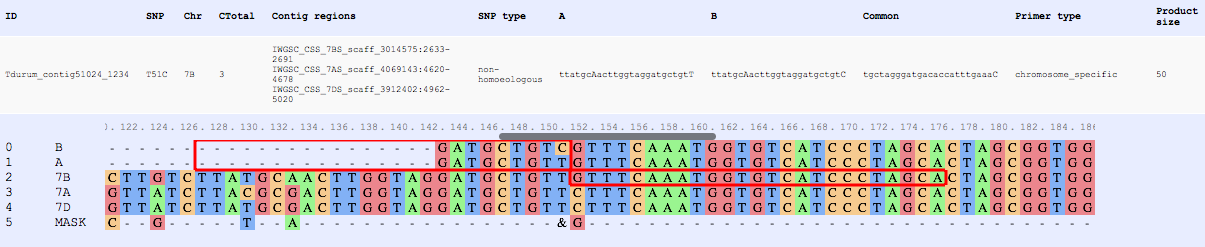
\includegraphics[width=0.75\textwidth]{PolyMarker/Figures/website/non-hom-sp.png}
\end{subfigure}
\begin{subfigure}{1\textwidth}
\caption{}
\centering
\label{fig:poly:hom-sp}
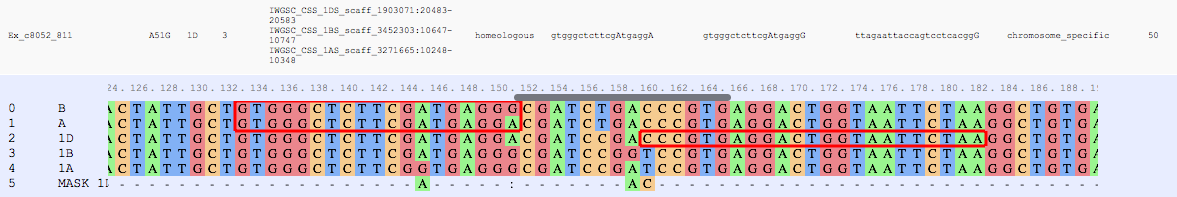
\includegraphics[width=0.75\textwidth]{PolyMarker/Figures/website/hom-sp.png}
\end{subfigure}
\begin{subfigure}{1\textwidth}
\caption{}
\centering
\label{fig:poly:hom-multi}
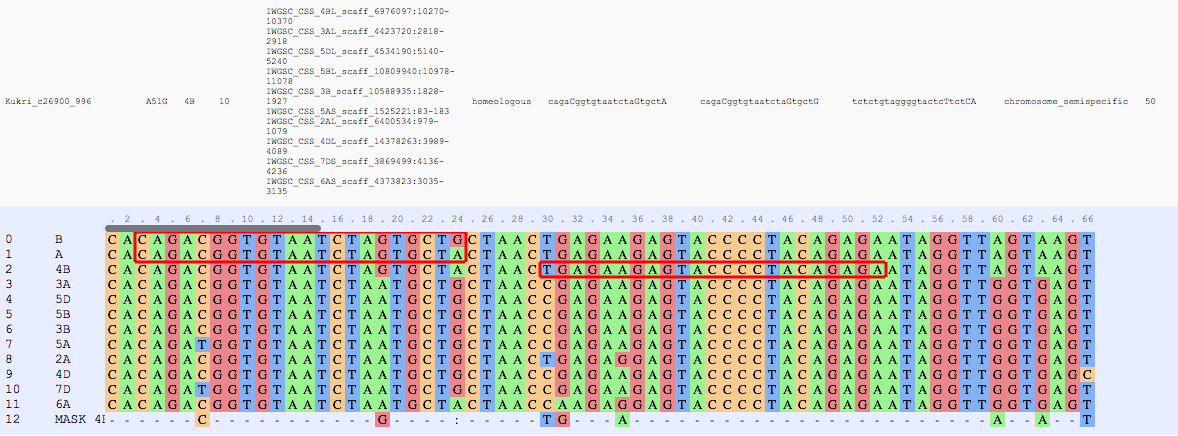
\includegraphics[width=0.75\textwidth]{PolyMarker/Figures/website/hom-multi.png}
\end{subfigure}
\caption[Examples outputs from the PolyMarker website.]{Examples outputs from the PolyMarker website. (\subref{fig:poly:non-hom-sp}) The primer triplet is genome specific. The original marker sequence had the SNP near the beginning of the template, but PolyMarker used the genomic reference to complement the sequence. (\subref{fig:poly:hom-sp}) An specific primer, but the SNP is located on the same position than an homologous variation. (\subref{fig:poly:hom-multi}) A case where the marker sequence align to 10 different chromosomes. The SNP is also located on a position with variations between genomes.}
\label{fig:poly:website}
\end{sidewaysfigure}


\section{Applications of PolyMarker}
Besides the project described in Chapter \ref{yr15}, PolyMarker has been used to design KASP primers for the wheat community.


\subsection{KASP assays for public sets of SNPs} 

PolyMarker was used to design KASP assays for the 81,587 markers from \citep{Wang2014}, available on the PolyMarker website and in CerealsDB \citep{Wilkinson2012}. 
Of those markers, 40,267 where designed based on the target chromosome from the genetic map provided in \citet{Wang2014}.  
Genes without a genetic position were aligned to scaffolds sorted by chromosome arms from the International Wheat Genome Sequencing Consortium \citep{Mayer2014} with BLAT \citep{Kent2002} and the best hit was selected as the putative location. 
97.5\% of the assays where designed and 76\% of them are semi-specific or specific, thereby improving their expected performance with respect to randomly designed primers (Table \ref{tab:poly:designed}). 
The pre-designed markers have been taken up by the community, for example, a subset of the designed assays was used to genotype a mapping population to find resistance to Fusarium head blight \citep{Burt2015}. 

\begin{table}

\centering
\caption{Count of KASP assays designed for the 40,267 SNP markers located in the genetic map from \cite{Wang2014}. 4,228 assays did not align to the target chromosome.  Not designed: Primer3 could not find viable primers flanking the SNP.}
\label{tab:poly:designed}

%\center
\begin{tabular}{rccc}

\toprule
 & Homoeologous  &     Varietal  & Percentage\\
  &  variant &      SNP & \\
 \midrule
Non-specific&1,765&5,857&21.15\%\\
Semi-specific&7,942&6,907&41.20\%\\
Specific&6,813&5,957&35.43\%\\
Not designed &242&556&2.21\%\\
\midrule
 Total&16,762&19,277&36,039\\
\bottomrule
\end{tabular}

\end{table}

Also, PolyMarker was used to design KASP assays for the 820K SNP Axiom array described in \citet{Winfield2016}. 
Briefly, the original set contains 819,556 SNPs called from exome capture on 43 bread wheat accessions and wheat relatives. 
Of those, 616,525 where mapped with \verb|exonerate| \citep{Slater2005} to the \acrshort{css} scaffolds. 
Of those, 86.1\% have an specific or semi-specific assay (Table \ref{tab:poly:designed820k}. 
This set of primers is also available in CerealsDB and it provides a valuable resource to groups that want to genotype using a subset of SNPs in the array, without the need to run the complete Axiom array.
This is especially relevant in breeding programmes who might want to run a small subset of markers linked to their favourite traits. 
The fact that the assays could be downloaded all in one makes it difficult to document the impact, but based on conversation with molecular breeders we are aware that they are being implemented in several breeding companies. 


\begin{table}

\centering
\caption{Count of KASP assays designed for the 616,525 SNP markers located to a \acrshort{css} scaffold from the 819,556 SNPs from \cite{Winfield2016}   Not designed: Primer3 could not find viable primers flanking the SNP.}
\label{tab:poly:designed820k}
\begin{tabular}{rccc}
\toprule
 & Homoeologous  &     Varietal  & Percentage\\
  &  variant &      SNP & \\
\midrule
 Non-specific & 20,189                 & 56,516         & 12.44\%       \\
 Semi-specifc & 167,018                & 132,145        & 48.52\%       \\
 Specific     & 139,202                & 92,487         & 37.58\%       \\
 Not designed & 3,116                  & 5,852          & 1.45\%        \\
 \midrule
 Total        & 329,525                & 287,000        & 616,525      \\
\bottomrule
\end{tabular}
\end{table}


\subsection{SNPs in a mutant population}
\label{sub:poly:muts}
PolyMarker was used to design primers to validate SNPs in a Targeted Induced Local Lesions in Genomes (TILLING) population, an approach to identify the function of genes by mutating them. 
Briefly, wheat lines are mutated with ethyl methanesulphonate that produce G>A or C>T mutations. 
The initial mutation is called $M_{1}$ and each plant is self-pollinated to fix the mutations. 
The second generation is called $M_{2}$, and so on. 
With each generation the mutations, which were originally heterozygous, get fixed and become homozygous. 
In the process, some mutations are lost. 
For this experiment, three $M_{5}$ lines were sequenced with exome capture. 
The purpose of the experiment was to assess the feasibility of exome capture for call for SNPs.  

To validate the SNPs detected at different levels of coverage and allele frequencies 150 assays were designed.
The assays were tested on the $M_{5}$ used for SNP calling and on the progenitors at $M''$, $M_{3}$. 
Most of the SNP calls with more than 8 variant calls or an allele frequency over 0.8 were validated (Table \ref{tab:poly:mutSummary}). 
At the same time, only 27\% of the SNPs with an allele frequency of 0.6 and 17\% of the cases with seven or less variant reads were successful. \citep{King2015}. 
On this experiment PolyMarker was useful on validating and calibrating the minimum coverage to call SNPs reliably. 


\begin{table}

\centering
\caption{Summary table of the validation of candidate SNPs by KASP marker assays. Candidate SNPs are classified by number of supporting variant reads or by allele frequency and validataed by KASP assays. Table from \citet{King2015}.}
\label{tab:poly:mutSummary}

\begin{tabular}{llrrl}
\toprule
 Criterion        & Number/   &   KASP  &   Validated  & Validated   \\
          & Frequency   &    assays &    SNPs &  (\%)   \\
\midrule
Variant reads     & 4                  &            25 &                1 & 4\%              \\
                  & 5                  &            17 &                3 & 18\%             \\
                  & 6                  &            14 &                2 & 14\%             \\
                  & 7                  &            14 &                3 & 21\%             \\
                  & 8                  &            10 &                5 & 50\%             \\
                  & 9                  &            12 &                9 & 75\%             \\
                  & \ensuremath{>}10                &            35 &               29 & 83\%             \\
\midrule
 Allele frequency & 0.2                &            51 &                2 & 4\%              \\
                  & 0.4                &            27 &               13 & 48\%             \\
                  & 0.6                &            18 &                9 & 50\%             \\
                  & 0.8                &             3 &                2 & 67\%             \\
                  & 1                  &            31 &               27 & 87\%             \\
\bottomrule
\end{tabular}
\end{table}

%TODO: Add more details as suplemental?
On a follow-up experiment consisting of 1,200 Cadenza (Hexaploid) and 1,535 Kronos (Tetraploid) wheat lines \citep{Krasileva2016} over 250 SNPs were experimentally validated where also validated. Genome-specific primers were designed for 172 and 80 SNPs in the Cadenza and Kronos populations, respectively. These mutations were spread across 19 and 8 $M_{4}$ Cadenza and Kronos lines respectively. 
Of those, 71(85.5\%) Kronos and 147(88.8\%) of the Cadenza primers where valid assays, consistent with the pilot study (Tables \ref{app:PolyMarkerM4ValidationCadenza} and \ref{app:PolyMarkerM4ValidationKronos}).  

\section{Modifications of PolyMarker}
PolyMarker is not restricted to wheat or to KASP assays, the source code is flexible and can be extended for other types of analyses. 
On each of the following projects, PolyMarker has been adapted to design primers in species where KASP has not been used before, the primers are used for regular PCR amplification, or the use of KASP is not the conventional SNP calling. 

\subsection{Deletions on a mutant population}
%Algorithm to produce KASP for deletions in polyploids. 
\label{poly:dels}  

On some of the TILLING mutant lines, long deletions spanning multiple scaffolds were detected \citep{Krasileva2016}.
To validate the deletions it is possible to use KASP assays to produce primers that amplify homoeologues.  
PolyMarker was modified to search for variations across homoeologues to select a common primer that will amplify two genomes (Figure \ref{fig:poly:wt}, \subref{fig:poly:homM4}; reverse primer). 
On lines without the targeted deletion, the amplification corresponds to an heterozygous assay with equal signal for both the A and the B allele (Figure \ref{fig:poly:homFalse}).  
When a deletion is present the results of the assay resemble the results for a homozygous individual, with the intensity of the assay towards the the conserved homoeologue (Figure \ref{fig:poly:homReal}).

\begin{figure}
    \centering
    \begin{subfigure}[b]{0.45\textwidth}
        \caption{}
        \centering
        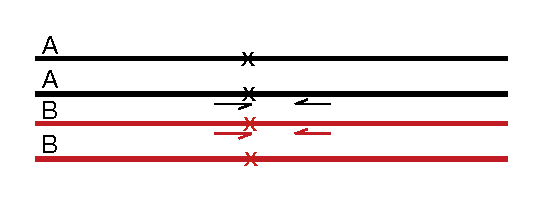
\includegraphics[width=1\textwidth]{PolyMarker/Figures/deletions/wt.pdf}
        \label{fig:poly:wt}
    \end{subfigure}
    ~
     \begin{subfigure}[b]{0.45\textwidth}
        \caption{}
        \centering
        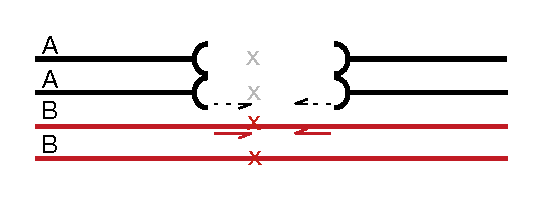
\includegraphics[width=1\textwidth]{PolyMarker/Figures/deletions/homM4.pdf}
        \label{fig:poly:homM4}
    \end{subfigure}
    \begin{subfigure}[b]{0.3\textwidth}
        \caption{}
        \centering
        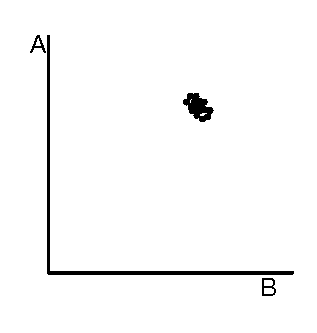
\includegraphics[width=1\textwidth]{PolyMarker/Figures/deletions/homFalse.pdf}
        \label{fig:poly:homFalse}
    \end{subfigure}
    ~
    \begin{subfigure}[b]{0.3\textwidth}
        \caption{}
        \centering
        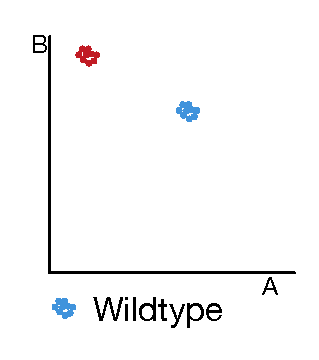
\includegraphics[width=1\textwidth]{PolyMarker/Figures/deletions/homReal.pdf}
        \label{fig:poly:homReal}
    \end{subfigure}
    \caption[KASP assays to validate homozygous deletions.]{KASP assays to validate homozygous deletions. (\subref{fig:poly:wt}) Primer positions for wildtype. Red and black indicate the A and B genome respectively. Primers are indicated by arrows with the target homoeologous SNP marked by an "X"(\subref{fig:poly:homM4}) Primer positions on  homozygous deletion on $M_{4}$ (\subref{fig:poly:homFalse}) Heterozygous amplification on wildtype DNA (no deletion), including both homoeologues. (\subref{fig:poly:homReal}) Homozygous amplification on deletion line, only the non-deleted homoeologue is amplified. }
\end{figure}

To be able to select primers that will amplify two homoeologues, the default scoring values (Listing \ref{lst:poly:defScore}) are changed. 
The altered scoring gives priority in the following order semi-specific, non-specific and specific. 
The rest of the pipeline is unaltered, showing that the modular design allows to add new functionality without breaking the pipeline. 

\begin{code}[language=Ruby,caption=Score values to select semi-specifc primers, label=lst:poly:delsScore]
kasp_container.scores[:chromosome_specific] = 0
kasp_container.scores[:chromosome_semispecific] = 1000
kasp_container.scores[:chromosome_nonspecific] = 100    
\end{code}

A set of KASP assays for the the deletions and mutations located on the same chromosome where designed to validate 11 homozygous deletions on $M_{4}$ plants. 
In all cases the segregation of the mutations was as expected, except for a predicted heterozygous mutation that was called as homozygous. 
Also, all the KASP assays that contained a deletion were called homozygous, as expected. 
To ensure that the calls did not come from a single cluster, 4 wildtype plants were genotyped and the markers for deletions where called as heterozygous. 
An example of a validated deletion and the surrounding mutations, with the calls for each individual is shown on Table \ref{app:poly:homDelCad0423}. 
  

\begin{sidewaystable}
\centering
\caption{Validation of homozygous deletions on line Cadenza0423. }
\label{app:poly:homDelCad0423}
\begin{localsize}{6}{7}
\begin{tabular}{llllrllllllllllllllll}
\toprule
 Marker                                   & Deletion           & chr   &     cM & 1   & 2   & 3   & 4   & 5   & 6   & 7   & 8   & 9   & 10   & 11   & 12   & C   & C   & C   & C   & Result       \\
\midrule
 5BS\_2297308\_Cadenza0423\_12664\_C12664T    & -          & 5B    &  4.551 &  X   & X   & -   & X   & X   & X   & X   & X   & X   & X    & -    & X    & Y   & Y   & Y   & Y   & HOM Mutation \\
 5BL\_10812849\_Cadenza0423\_5664\_G5664T     & -          & 5B    & 38.769 &  X   & X   & -   & X   & X   & X   & X   & X   & X   & X    & -    & X    & Y   & Y   & Y   & Y   & HOM Mutation \\
 5BL\_10825062\_Cadenza0423\_7917\_G7917A     & -          & 5B    & 38.769 &  X   & X   & -   & X   & X   & X   & X   & X   & X   & X    & -    & X    & Y   & Y   & Y   & Y   & HOM Mutation \\
 IWGSC\_CSS\_5BL\_scaff\_10847976:27068-27231 & +          & 5B    & 38.769 &  X   & X   & -   & X   & X   & X   & X   & X   & X   & X    & -    & X    & H   & H   & H   & H   & Hom Deletion \\
 IWGSC\_CSS\_5BL\_scaff\_10847976:28118-28674 & +          & 5B    & 38.769 &  X   & X   & -   & X   & X   & X   & X   & X   & X   & X    & -    & X    & H   & H   & H   & H   & Hom Deletion \\
 IWGSC\_CSS\_5BL\_scaff\_10865441:15863-15946 & +          & 5B    & 38.769 &  X   & X   & -   & X   & X   & X   & X   & X   & X   & X    & -    & X    & H   & H   & H   & H   & Hom Deletion \\
 5BL\_10837222\_Cadenza0423\_4616\_G4616A     & -          & 5B    & 39.905 &  X   & X   & -   & X   & X   & X   & X   & X   & X   & X    & -    & X    & Y   & Y   & Y   & Y   & HOM Mutation \\
 5BL\_10891320\_Cadenza0423\_18847\_C18847T   & -          & 5B    & 45.594 &  Y   & Y   & -   & Y   & H   & X   & X   & Y   & H   & Y    & -    & H    & Y   & Y   & Y   & Y   & HET Mutation \\
\bottomrule
\end{tabular}
\end{localsize}
\end{sidewaystable}

\subsection{Genotyping \textit{Puccinia 
striiformis} f. sp. \textit{tritici} isolates.}
In \cite{Hubbard2015}, \gls{pst} isolates were sequenced and assigned to clusters, according to their genotype.
The clusters are useful to monitor the changes in the pathogen population, which can be used to predict if certain wheat lines will be resistant to the isolates in the field. 
\gls{pst} is a dikaryon, an organism with two nuclei, each one containing a single haploid chromosome.
For PolyMarker it can be treated as a diploid, so the \verb|--genomes_count 1| argument was used.
PolyMarker was used to design primers for \gls{pst}, using the assembly PST-130 \citep{Cantu2011}.
As the assembly is fragmented, an \textit{ad hoc} function was used to always get the name of the assembly (Listing \ref{lst:poly:pst130}). 
Out of 15 assays, 11 can be used to identify to which cluster of isolates a sample is likely to belong, Table \ref{app:PolyMarkerPST}.
Until this study, the previous method to genotype \gls{pst} was \gls{ssr} markers which were difficult to replicate across laboratories and interpret in cases of multiple alleles \citep{Ali2014}.

\begin{code}[language=Ruby,caption=Function that always returns PST130 as chromosome, label=lst:poly:pst130]
arm_selection_functions[:pst130] = lambda do |contig_name|       
  return "PST130"
end
\end{code}


\begin{sidewaystable}
\centering
\caption{PolyMarker used to genotype PST. The X and Y represent the the two possible allels.  X:X and Y:Y correspond to homozygous call of the corresponding allele. X:Y correspond to heterozygous calls. The '-' symbol correspond to failed assays. }
\label{app:PolyMarkerPST}
\begin{localsize}{9}{10}

\begin{tabular}{rlrll|cc|cc|ccc|cc}
\toprule
          &              &  &  & & \multicolumn{2}{c}{Cluster I isolates}        & \multicolumn{2}{c}{Cluster II isolates}        & \multicolumn{3}{c}{Cluster III isolates}         & \multicolumn{2}{c}{Cluster IV isolates}        \\
Assay & Contig       & Position &  X &  Y & 13/26              & 13/123 & CL1                 & T-13/3 & 13/09                & 13/23 & 13/182 & 13/36               & 13/40 \\
 \midrule
  1  & PST130\_14470 & 268      & C        & T        & X:Y                & X:Y    & X:X                 & X:X    & X:X                  & X:X   & X:X    & X:X                 & X:X   \\
  2  & PST130\_8160  & 11876    & C        & T        & Y:Y                & Y:Y    & X:Y                 & X:Y    & X:Y                  & X:Y   & X:Y    & X:Y                 & X:Y   \\
  3  & PST130\_14628 & 1712     & A        & C        & X:Y                & -      & X:X                 & X:X    & X:X                  & X:X   & X:X    & X:X                 & X:X   \\
  4  & PST130\_14898 & 503      & G        & A        & X:X                & X:X    & X:Y                 & X:Y    & X:Y                  & X:Y   & -      & X:Y                 & X:Y   \\
  5  & PST130\_28344 & 2372     & A        & G        & Y:Y                & Y:Y    & X:Y                 & X:Y    & Y:Y                  & Y:Y   & Y:Y    & Y:Y                 & Y:Y   \\
  6  & PST130\_7634  & 3463     & A        & C        & Y:Y                & Y:Y    & X:Y                 & X:Y    & Y:Y                  & Y:Y   & Y:Y    & Y:Y                 & Y:Y   \\
  7  & PST130\_7629  & 11699    & G        & A        & Y:Y                & Y:Y    & X:Y                 & X:Y    & Y:Y                  & Y:Y   & Y:Y    & Y:Y                 & Y:Y   \\
  8  & PST130\_10943 & 2979     & C        & T        & X:Y                & X:Y    & X:Y                 & X:Y    & X:X                  & X:X   & X:X    & X:Y                 & X:Y   \\
  9  & PST130\_10126 & 6216     & G        & T        & Y:Y                & Y:Y    & X:X                 & X:X    & X:X                  & X:X   & -      & Y:Y                 & Y:Y   \\
  10 & PST130\_22010 & 172      & C        & T        & Y:Y                & Y:Y    & Y:Y                 & Y:Y    & X:Y                  & X:Y   & -      & X:Y                 & X:Y   \\
  11 & PST130\_16961 & 1098     & C        & T        & X:X                & X:X    & X:Y                 & X:Y    & Y:Y                  & Y:Y   & Y:Y    & X:Y                 & X:Y   \\
  12 & PST130\_6915  & 2710     & A        & T        & Y:Y                & Y:Y    & Y:Y                 & Y:Y    & Y:Y                  & X:Y   & X:Y    & Y:Y                 & Y:Y   \\
  13 & PST130\_12479 & 1428     & C        & T        & X:X                & X:X    & Y:Y                 & Y:Y    & X:X                  & X:X   & X:X    & Y:Y                 & X:X   \\
  14 & PST130\_7634  & 3883     & C        & G        & X:X                & X:X    & X:Y                 & X:Y    & X:X                  & X:X   & X:Y    & X:Y                 & X:X   \\
  15 & PST130\_14470 & 456      & T        & C        & Y:Y                & Y:Y    & X:Y                 & X:Y    & Y:Y                  & Y:Y   & X:Y    & Y:Y                 & Y:Y   \\
\bottomrule
\end{tabular}
\end{localsize}
\end{sidewaystable}


\section{Discussion}



%Perhaps cite some of the paper I showed you which used the dioploid progenitors, etc to do this. You need a reference to say this somewhere. Also you might want to extend this a bit. 

%Look at Figure 1 in this paper:
%https://bmcgenomics.biomedcentral.com/articles/10.1186/1471-2164-11-702

%this might provide you an idea of what you coudl say was the status quo before you started and where you left the field.  Especially the use of nullisomics.. include the info on Table 1 since this is important in terms of primer design

%Other papers to mention:
%http://www.nrcresearchpress.com/doi/abs/10.1139/g09-033#.V-RKDTXwmec

%And probably importantly is the ISBP markers which are beased on retro junctions.. so you can spend a paragraph discussing how these work and the advantage of being able to use RNAseq and exome capuer data to do yours, as opposed to ISBP..http://onlinelibrary.wiley.com/doi/10.1111/j.1467-7652.2009.00477.x/full

Before the \gls{css} assembly, which has scaffolds assigned to a chromosome arm, the design and validation of genome-specific primers for polyploid wheat was a labour intensive process (Figure \ref{fig:poly:oldGSP}; \citealt{Akhunov2010}). 
Briefly, the steps to develop primers for wheat was: 

\begin{enumerate}
    \item \textbf{Find candidate ESTs} from a database. This could be the UniGene database from the \gls{ncbi} or gene sequences from a relative species, such as \textit{Brachypodium distachyon}.
    \item \textbf{Design primers from UniGenes.} The sequence of the ESTs used as a reference are aligned across them. The conserved regions are used to design primers to be able to amplify the same region across different species.
    \item \textbf{\gls{pcr} amplification of diploid species.} DNA from \textit{T. urartu}, \textit{Ae. tauschii} and, \textit{Ae. speltoides} are used to amplify the identified sequences. 
    \item \textbf{Sequence the amplicons}. The \gls{pcr} products from the relative species are sequenced individually with capillary sequence. 
    \item \textbf{Alignment of the amplicons}. To search for variations between related species, the amplicons are aligned and the bases that are different across diploid species are used to design new primers, that should be genome specific in hexaploid wheat. 
    \item \textbf{Validation on nullisomic-tetrasomic lines}. 
Those research lines have been treated to remove one of their chromosome pairs. 
In the process, one of the homoeologue chromosomes is duplicated (four chromosomes, hence tetra).
This lines are useful to evaluate the effect of a particular chromosome. 
In the case of genome-specific primer design, it is possible to evaluate if the primer is specific to the missing chromosome, as it will not amplify in the nullisomic-tetrasomic line. 
If the primer amplifies it means that it is not specific to the target chromosome 
(Figure \ref{fig:poly:nullitetra}).
\end{enumerate}

\begin{figure}
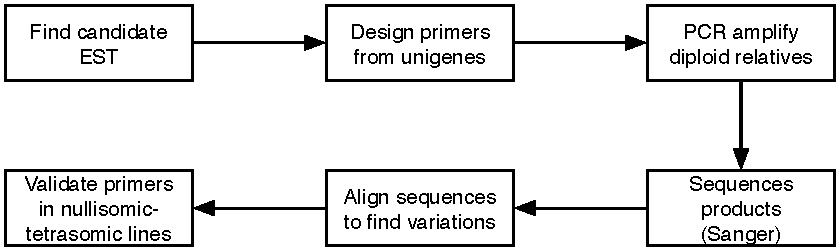
\includegraphics[width=1\textwidth]{PolyMarker/Figures/disc/OldGSP.pdf}
\caption{Previous process of primer design and validation}
\label{fig:poly:oldGSP}
\end{figure}

\begin{SCfigure}
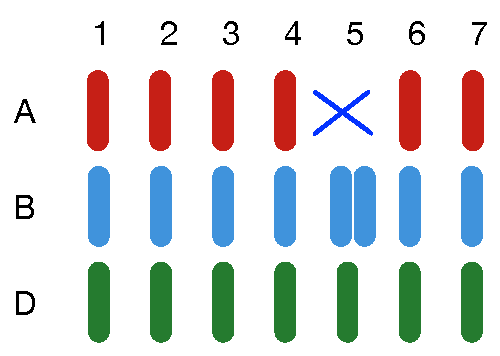
\includegraphics[width=0.65\textwidth]{PolyMarker/Figures/disc/NulliTera.pdf}
\caption[Nullisomic-tetrasomic lines]{ Nullisomic-tetrasomic lines. This example has chromosome 5A missing and 5B duplicated. }
\label{fig:poly:nullitetra}
\end{SCfigure}

Even having a the sequence for each homoeologue, without an automated bioinformatic pipeline, the primer design was done manually, a slow, error-prone and, repetitive process. 
The steps require the use of several bioinformatics tools, but once I understood the primer design steps I decided to automate the process. 
Since designing genome-specific primers is a common task in wheat research and breeding, the community showed interest on the tool and I decided to refine it and make it open source. 
PolyMarker has been used successfully in several projects \citep{Ramirez-Gonzalez2015b,Hubbard2015,Burt2015,King2015,Sollars2016} and it even allowed the novel use of KASP assays to validate long deletions in polyploids \citep{Krasileva2016}. 
 
As a common source of SNPs are gene models, designing primers directly from the sequence flanking the SNP may run over the intron-exon junctions, producing primers that will not amplify on genomic DNA. 
To be able to use DNA I had to identify on which hit the SNP was located, the internal coordinate and a mapping coordinate to the original sequence. 
With this dual coordinate system I was able to design primers in the genome space, even when the origin was a transcript. 

In order to be able to represent more than one base at the same tame, the IUAPC ambiguity codes \citep{Cornish-Bowden1985} were useful in the development of PolyMarker. 
With an ambiguity code, the template for the search can contain the SNP. 
Also, the codes were useful when representing all the observed bases on each coordinate in the local alignment. 

%\unsure{Look at http://www.ncbi.nlm.nih.gov/pmc/articles/PMC3868579/ to get some way to compare SRR vs SNP markers }

The ideas behind PolyMarker had been taken by other projects like the scripts described in \cite{Ma2015} and the corresponding web interface, GSP \citep{Wang2016}. 
Briefly, GSP does uses \verb|blast| to search in a local database to find all the homoeologous regions and provides a diagram with the bases that are genome specific. 
It then allows the user to select a primer pair according to the constrains for their individual experiment, like product size. 
The advantage over PolyMarker is that it allows to pick arbitrary primers, at the cost of having a step for manual selection of the pair. 
Recently, LGC also developed a program (MAGICBOX) that require a SNP sequence, does the alignment and selects primers with a genome specific anchor. 
As PolyMarker, it produces a local alignment with the genome-specific bases \citep{Curry2016} and a mask highlighting the variations providing the specificity to the primer.
On personal communications in conferences I had found out that LGC, the company behind KASP, uses PolyMarker to design primers. Also Bayer has an in house implementation of the algorithm. 

As the code is open source, anyone can see the implementation details and extend the code for different types of primers. 
A successful modification to PolyMarker was to be able to design primers to detect homozygous deletions with KASP assays, despite the fact that neither KASP or PolyMarker were designed for deletions. 
The modularity of the code permits to swap components with relatively little effort. 

The current web interface of PolyMarker is limited to KASP assays, however the command line version is more flexible and has been used to design primers for PCR amplicons, capillary sequencing and on other organisms. 
However, to install the command requires a Linux machine and some knowledge on the command line. 

PolyMarker is a tool that was originally designed to design the markers to validate the \glspl{snp} found in Chapter \ref{yr15}. 
Overall, PolyMarker provides an useful resource to the wheat community, as the primer design process is now streamlined. 
PolyMarker is not restricted to wheat, it can be used on any polyploid systems, like the polyploids in the genus \textit{Brassica}.
As new references of wheat come available, PolyMarker should be updated to work with pseudo-molecules and the web interface updated accordingly. The source code of PolyMarker is open source and available on \url{https://github.com/TGAC/bioruby-polyploid-tools}. 
